\documentclass[conference]{IEEEtran}
\IEEEoverridecommandlockouts
% same look as our earlier arXiv papers (IEEEtran, Times, bold run-in headings); XeTeX via tectonic for Devanagari
\usepackage{fontspec}
\setmainfont{texgyretermes}[Extension=.otf, UprightFont=*-regular, BoldFont=*-bold, ItalicFont=*-italic, BoldItalicFont=*-bolditalic]
\newfontfamily\devanagarifont[Script=Devanagari]{Kohinoor Devanagari}
\newcommand{\np}[1]{{\devanagarifont #1}}
\usepackage{microtype}
\usepackage{graphicx}
\usepackage{booktabs}
\usepackage{amsmath,amssymb}
\usepackage{xcolor}
\usepackage[numbers,sort&compress]{natbib}
\usepackage{url}
\usepackage{xurl}
\usepackage[hidelinks]{hyperref}
\makeatletter\renewcommand{\paragraph}[1]{\par\noindent\textbf{#1}\hspace{0.5em}}\makeatother
\renewenvironment{abstract}{\par\noindent\footnotesize\bfseries\textit{Abstract.}\ }{\par\vspace{0.6\baselineskip}}
\newcommand{\artifactnote}{Code, frontend, evaluation scripts and results: \url{https://github.com/Naamche-Labs/swar} (to be published with the paper).}

\begin{document}

\title{Swar: Open Zero-Shot Voice Cloning for Nepali from Phone-Quality Speech}

\author{
\IEEEauthorblockN{Aarjan Chaudhary}
\IEEEauthorblockA{\textit{Naamche Labs}}
}

\maketitle

\begin{abstract}
Nepali has about 32 million speakers and almost no open text-to-speech that sounds like a person from Nepal. We present Swar, an open zero-shot voice cloning system for Nepali built on F5-TTS initialised from IndicF5 and adapted with Nepal-recorded speech, 50 hours of English and 2.5 hours of conversational podcast speech. Most of the gain comes from parts that need no extra training: a text frontend that writes Nepali as it is spoken in Nepal and English the way Nepali speakers say it, enrolment that turns casual voice notes into prompts with transcripts from a Nepali telephony recogniser, and take selection that checks pronunciation, including word-final vowels measured in the audio, before voice similarity. On NepTTS-Bench, Swar's pronunciation error is 2.9\%, against 4.3\% for OmniVoice with the same prompt and 8.1\% to 17.0\% for the open and commercial systems with published audio. Clones of unseen speakers are accepted by two speaker verifiers as often as the speakers' own second recordings, and from 20 to 30 seconds of a WhatsApp voice note the clone is close to the person's held-out real speech. On FLEURS it is first on error rate, speaker similarity and predicted naturalness. On NepTTS-Bench no single prompt leads on both pronunciation and predicted naturalness: the demo voice, from a podcast speaker, reaches the highest UTMOS of any system at a higher pronunciation error than the studio voice. We report two negative results in detail. Speaker fine-tuning adds almost nothing over prompting, and for full English sentences the objective scores preferred a route that a native listener rejected. We release the model, the frontend, the enrolment pipeline and a demo.
\end{abstract}

\section{Introduction}

Nepali text-to-speech today is either closed (ElevenLabs, Google), built for one fixed voice (TingTing, Piper, Edge), or part of a multilingual Indic model whose Nepali was read mostly by speakers in India (IndicF5~\citep{indicf5}, Indic Parler-TTS~\citep{parler,indicparler}, Indic-Speak). A person in Kathmandu who wants a voice that sounds like their own, or like a neighbour, has no open option.

Three gaps follow. The first is pronunciation. Nepal Nepali says \np{श}, \np{ष} and \np{स} alike, starts words with ``b'' for \np{व}, and keeps word-final vowels that Indian-recorded data drops, so \np{खान} (``to eat'', said \emph{khaana}) comes out as ``khan''. The second is English. Everyday Nepali is full of English words, and a model that reads Nepali letters says them with Nepali sounds unless the spelling is right. The third is the audio people actually have: compressed voice notes with no transcript, often several speakers, recorded months apart.

\paragraph{Research questions.} We organise the study around four questions, answered in Section~\ref{sec:results}:
\begin{enumerate}
  \setlength\itemsep{0pt}
  \item \textbf{RQ1: Pronunciation.} How does Swar's pronunciation compare with open and commercial Nepali systems on a public benchmark?
  \item \textbf{RQ2: Cloning from phone audio.} How close is a clone made from a short, unlabelled voice note to the person's real held-out speech?
  \item \textbf{RQ3: Frontend.} How much do the Nepal pronunciation layer, the held final vowels and the English layer contribute?
  \item \textbf{RQ4: Training vs prompting.} Does fine-tuning on a speaker's own speech improve a voice beyond prompting with it?
\end{enumerate}

\paragraph{Findings.} Swar has the lowest pronunciation error on NepTTS-Bench by a wide margin, and its clones of unseen speakers pass speaker verification as often as real second recordings. The text frontend accounts for much of the pronunciation gain, and the two most effective changes came from a listener's reports that we confirmed by measurement: held word-final vowels and English spellings. Speaker fine-tuning barely moved any metric. Swar is not the most natural-sounding system by an automatic predictor, and on full English sentences automatic scores and a native listener disagreed.

\paragraph{Contributions.} We make five contributions:
\begin{enumerate}
  \setlength\itemsep{0pt}
  \item A Nepal pronunciation frontend for a character-input TTS model, with a held-final-vowel rule found and checked by measuring audio rather than ASR text (\S\ref{sec:frontend}).
  \item An English layer that writes the 2000 most common English words the way Nepali speakers say them, with five sound rules, and evidence that spelling, not training, fixed full-English output (\S\ref{sec:english}).
  \item A pronunciation metric for Nepali TTS that folds spelling differences speech does not carry, applied identically to every system (\S\ref{sec:setup}).
  \item An automatic enrolment and take-selection pipeline for phone-quality uploads, and results on a public benchmark, a studio test with a human ceiling, unseen-speaker cloning, code-switching and eight preset voices (\S\ref{sec:results}).
  \item Open weights, code and a demo.\footnote{\artifactnote}
\end{enumerate}

\section{Background and Related Work}

\subsection{Zero-Shot Text-to-Speech}
Zero-shot TTS clones a voice from a short prompt recording. Neural codec language models~\citep{valle} and multilingual systems such as YourTTS~\citep{yourtts}, XTTS~\citep{xtts} and CosyVoice~\citep{cosyvoice} predict discrete speech tokens. MaskGCT~\citep{maskgct}, E2 TTS~\citep{e2tts} and F5-TTS~\citep{f5} instead generate speech non-autoregressively from the prompt audio and its transcript; F5-TTS uses flow matching over mel spectrograms and a separate vocoder such as Vocos~\citep{vocos} or BigVGAN~\citep{bigvgan}. These models need an exact transcript of the prompt, which casual uploads do not come with.

\subsection{Indic and Nepali TTS}
IndicF5~\citep{indicf5} trains F5-TTS on Indic languages with character input; IndicVoices-R~\citep{indicvoicesr} supplies most of its Nepali, recorded largely in India. Fixed-voice systems include VITS-style models~\citep{vits} and description-controlled Parler-TTS~\citep{parler}, whose Indic version~\citep{indicparler} has one Nepali voice. For Nepal-recorded data, OpenSLR provides a studio TTS corpus~\citep{slr43} and crowd-sourced ASR speech~\citep{slr54}, and FLEURS~\citep{fleurs} adds multi-speaker read Nepali. Prior Nepali TTS is mostly single-voice concatenative or parametric synthesis; we are not aware of an open Nepali system that clones voices from phone audio.

\subsection{Evaluating Nepali TTS}
NepTTS-Bench~\citep{neptts} is the public Nepali benchmark: designed sentences in categories such as minimal pairs, questions and robustness, ASR-based character error, and a naturalness predictor. Automatic naturalness scores such as UTMOS~\citep{utmos} are trained on English read speech; we use them, but treat a native listener's judgement as the arbiter where the two disagree.

\section{System}\label{sec:system}

\subsection{Acoustic Model and Training Stages}
Swar is F5-TTS Base (336M parameters) with character input, initialised from IndicF5. Training ran in stages: (a) 130 h of IndicVoices-R and Rasa with verbatim transcripts; (b) 338 h adding IndicVoices read and extempore speech, with telephone-band conversation removed; (c) a read-speech polish; (d) an accent stage on 70.7 h of Nepal-recorded speech (OpenSLR 43/54, 545 speakers) plus Rasa; (e) a bilingual stage adding 50 h of LibriTTS-R English~\citep{librittsr} and 110 h of Nepal speech (6 epochs, learning rate $2\times10^{-5}$); and (f) a voices stage on 2.5 h of conversational podcast speech from ten speakers, used with their permission, with FLEURS and LibriTTS-R replay so that cloning and English are kept (11 epochs, $2\times10^{-5}$). Podcast pieces were cut at pauses and kept when they were typical of the speaker (ECAPA~\citep{ecapa} similarity to the speaker centroid $\geq 0.55$), cleaner than the speaker's worst 30\% by UTMOS, and transcribed with confidence $\geq 0.80$. Training on an H200 was numerically unstable for this model (non-finite gradients and noise output), while the same data on RTX PRO 6000, L4 and A100 was not.

\subsection{Text Frontend}\label{sec:frontend}
The model reads characters, so pronunciation is controlled by what it is given to read. The frontend applies, in order, mined respellings, held final vowels, Nepal pronunciation and the English layer, all to the model input only.

\paragraph{Nepal pronunciation.} Much of the training audio is Indian Nepali, where \np{श} and \np{ष} are ``sh'' and \np{व} is ``v''. The layer writes words as they are said in Nepal: \np{दशचोटि}$\to$\np{दसचोटि}, \np{विशेष}$\to$\np{बिसेस}, \np{शिक्षा}$\to$\np{सिछ्या}.

\paragraph{Held final vowels.} A listener heard \np{खान} and \np{आज} said without their final vowel (``khan'', ``aaj''). A read-back ASR cannot see this, because its language model restores the expected word, so we measured the audio: forced alignment of the sentence with a literal Devanagari CTC model gives the duration of the word's final sound. Appending halanta+\np{अ} to a short word list and to verb forms ending in \np{ेर}, \np{एर} or \np{ैन} lengthens that sound (Fig.~\ref{fig:vowel}). A plain \np{अ} lengthened it more, but the listener heard it as distorted, so the halanta form is used and take selection checks the audio (\S\ref{sec:take}).

\subsection{English Layer}\label{sec:english}
Each English word gets a Devanagari spelling: a curated list first, then Google's Nepali lexicon, then CMUdict-derived candidates ranked by how often Nepali writers use each spelling (counts over 8.4M sentences). A native listener still heard full English as broken. The cause was the spellings. Some were Nepali words with other meanings: \emph{bought} \np{बाट} (``from''), \emph{that} \np{दात} (``tooth''), \emph{more} \np{मर} (``die''), \emph{former} \np{फार्मर} (``farmer''), \emph{wrong} \np{रङ} (``colour''). We reviewed the 2000 most common English words by hand, changing 339 spellings, and added five rules that cover the rest of the vocabulary: ``o'' before \emph{r} is \np{ओ} (\np{मोर}); a final \emph{z} after a consonant is \np{स} (\np{इयर्स}); \emph{-ed} after \emph{t}/\emph{d} and \emph{-es} after a sibilant keep their vowel (\np{नीडेड}, \np{चेन्जेज}); \emph{k}, \emph{p} and \emph{f} before \emph{s}, \emph{sh}, \emph{t} and \emph{ch} are joined (\np{इक्स्पेक्ट}, \np{सेफ्टी}); and English ``sh'' stays \np{श} (\np{शो}, not \np{सो}, which reads as ``so'').

\subsection{Enrolment from Uploads}
Uploads are cut at pauses into 3.5--10 s pieces. One speaker is kept by ECAPA clustering, or all pieces if the uploader says every clip is one person: one person's notes recorded months apart scored 0.51--0.60, the same range as two different people. Transcripts come from Kriti Telephony, a Nepali hybrid RNNT/CTC Conformer; on WhatsApp notes it matched hand transcripts where MMS~\citep{mms} and Whisper~\citep{whisper} did not. Three prompts are chosen by typicality, transcript confidence and naturalness, and the speaker's median pace sets the speaking rate. For the demo, Kriti's CTC head is exported to ONNX and runs in the same process as the TTS model with a reimplemented log-mel frontend, which gave identical transcripts on our checks.

\subsection{Take Selection}\label{sec:take}
Each sentence gets $N$ takes. Each take is read back; takes within 3 points of the lowest pronunciation error compete on similarity to the enrolled voice plus $0.1\times(\text{UTMOS}-3)$. In sentences with a held word, takes whose held sound is shorter than 120 ms are dropped first. Long text is spoken one sentence at a time, with 0.38 s after a full stop and 0.45 s after a question, because F5-TTS runs straight through a full stop inside one generation; one prompt is kept throughout so the voice does not drift between sentences.

\subsection{Vocoder}
A BigVGAN-v2 vocoder fine-tuned on F5's mel features (56k steps) scores copy-synthesis UTMOS 3.57 against 3.07 for Vocos on real speech, and 3.60 against 3.54 on TTS output. On phone-quality clones it scored lower (3.00 against 3.12), so Vocos stays the default for clones and BigVGAN is used for studio voices.

\section{Experimental Setup}\label{sec:setup}

\paragraph{Benchmarks.} NepTTS-Bench~\citep{neptts}: 205 scored sentences (the free-form natural speech category is skipped for every system). A studio test: 200 unseen Rasa test sentences in five styles, with the speakers' own recordings scored identically as a human ceiling. Unseen-speaker cloning: 50 IndicVoices-R speakers never seen in training (100 items), and FLEURS (82 items from Nepal speakers). Code-switching: 30 held-out Nepali sentences with English words, written before any output was heard. Phone audio: WhatsApp voice notes from consenting speakers, with held-out pieces the clone must match.

\paragraph{Systems.} Published audio of TingTing, ElevenLabs v3, Gemini and Piper on NepTTS-Bench, re-scored with our scorers; Indic-Speak (two Nepali voices) and Indic Parler-TTS (its only Nepali voice) generated with their model cards' defaults; OmniVoice with our prompts. All our runs use one take, a female studio prompt with pace calibration, and 16 flow steps unless stated.

\paragraph{Metrics.} Standard CER uses MMS-1b-all~\citep{mms} with its Latin tokens masked, because it otherwise switches script on names and English words, more on synthetic speech than on human speech. \emph{Pronunciation CER} additionally folds spellings that Nepali speech does not distinguish (\np{श/ष/स}, \np{ि/ी}, \np{ु/ू}, \np{व/ब}, \np{ण/न}, nasal forms, spacing and word-final halanta) and converts English words in references with our frontend, identically for every system and for human recordings. Speaker similarity is ECAPA-TDNN cosine; naturalness is UTMOS22 and NepTTS-Bench's public NepaliMOS; full-English intelligibility is Whisper-large-v3~\citep{whisper} WER. MMS-1b-all is licensed for non-commercial use and is used only for measurement.

\section{Results}\label{sec:results}

\subsection{RQ1: Pronunciation}
Table~\ref{tab:bench} and Fig.~\ref{fig:bench} give NepTTS-Bench results. Swar's pronunciation CER is 2.9\%; the next system is OmniVoice run with our studio prompt (4.3\%), then Indic-Speak Srijana (8.1\%) and ElevenLabs v3 (12.9\%). Among systems with published audio, Swar has the lowest pronunciation error in every benchmark category except newspaper ambiguities (4 sentences), where Indic-Speak Sagar is slightly lower (4.3 against 4.8). On standard CER Swar also leads, OmniVoice within 0.5 points. With the studio prompt, Swar does not lead on predicted naturalness: Indic-Speak Srijana scores UTMOS 3.97 and OmniVoice 3.93, against 3.82. With a read-style prompt in a podcast voice (Section~\ref{sec:voice}), Swar's demo voice Maya reaches UTMOS 4.09, the highest of any system, and beats Srijana on both error rates (7.45 and 4.52 against 10.25 and 8.12), but not OmniVoice (6.68 and 4.32). No single prompt leads on everything. The public NepaliMOS predictor puts every system between 2.88 and 3.05 (Swar 2.96, OmniVoice 2.98, Piper 3.05, Maya 2.88). The small paired differences are consistent across sentences, but the ranking does not follow intelligibility or the listener: Piper, with the most pronunciation errors, scores highest, and the voice our listener preferred scores lowest.

\begin{table}[t]\centering\small
\caption{NepTTS-Bench, 205 sentences: mean per-file CER (\%) and UTMOS. Our rows use today's frontend and one take; the Maya and Sabina rows use a read-style prompt chosen on development data. Other systems are their published or default-setting audio, scored identically.}\label{tab:bench}
\begin{tabular}{lrrr}\toprule
System & CER & Pron.\ CER & UTMOS\\\midrule
Swar, final model & \textbf{6.19} & \textbf{2.92} & 3.82\\
Swar, Maya voice & 7.45 & 4.52 & \textbf{4.09}\\
Swar, Sabina voice & 9.82 & 6.57 & 4.08\\
Swar, accent stage & 6.23 & 3.35 & 3.81\\
Swar, bilingual stage & 6.45 & 3.26 & 3.78\\
OmniVoice (our prompts) & 6.68 & 4.32 & 3.93\\
Indic-Speak Srijana & 10.25 & 8.12 & 3.97\\
Indic Parler-TTS Amrita & 11.70 & 9.51 & 3.26\\
Indic-Speak Sagar & 12.37 & 10.53 & 3.81\\
TingTing Subina & 13.39 & 11.25 & --\\
ElevenLabs v3 & 15.70 & 12.91 & --\\
Gemini & 15.31 & 15.03 & --\\
Piper & 18.68 & 17.00 & --\\\bottomrule
\end{tabular}
\end{table}

\begin{figure}[t]\centering
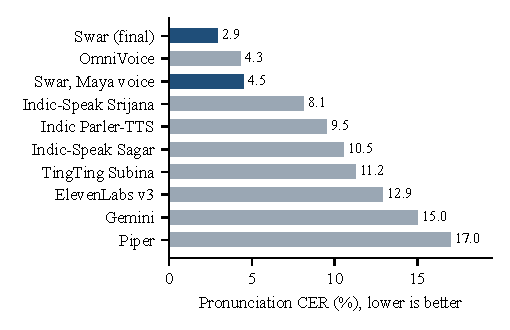
\includegraphics[width=\columnwidth]{fig_bench.pdf}
\caption{Pronunciation CER on NepTTS-Bench (lower is better).}\label{fig:bench}
\end{figure}

On the studio test, Swar's mean per-file CER is 8.95 against 10.93 for the human recordings of the same sentences (names: 22.1 against 21.9), with UTMOS 3.72 against 3.62. Against the real take of the same sentence, the clone's ECAPA similarity is 0.78, its F0 correlation 0.49, and its pace within 13\%.

\subsection{RQ2: Cloning from Phone Audio}
On 50 unseen IndicVoices-R speakers, ECAPA accepts 97\% of clones as the target speaker, against 98\% of genuine second recordings (equal error rate 2\%), and WavLM-SV~\citep{wavlm} accepts 91\% of both. On FLEURS, the final model reaches similarity 0.694 and CER 4.6, against 0.681 and 5.3 for OmniVoice, whose predicted naturalness is higher (UTMOS 2.49 against 2.39). FLEURS prompts are noisy (the real recordings score UTMOS 2.24) and the model copies the noise. Denoising the prompt with DeepFilterNet3~\citep{deepfilternet}, with the removal capped at 18\,dB (chosen on FLEURS validation speakers), gives CER 4.55, similarity 0.691 and UTMOS 2.67: first on all three. Full denoising sounds cleaner still (UTMOS $+0.3$ on validation) but costs similarity and CER.

On WhatsApp voice notes, the clone of a held-out sentence matches the person's real clip at 0.767, against 0.771 between that person's own clips, for a speaker with five minutes of notes; for a speaker whose notes were recorded months apart, the figures are 0.598 and 0.630. From a single 30-second window, similarity is 0.74, 0.70 or 0.62 depending on the window: slow, careful speech gave the lowest. Enrolment from a 30.6 s upload takes 23.5 s on one L4 GPU, and a best-of-4 sentence about 10 s.

\subsection{RQ3: The Frontend}
\paragraph{Pronunciation layers.} With the accent-stage model, adding the mined fixes, the Nepal pronunciation layer and the English layer lowered NepTTS-Bench pronunciation CER from 3.98 to 3.13 at unchanged standard CER (6.14 to 6.15), as expected for a layer whose effect is on sounds the standard metric does not separate. On the 30 code-switched sentences, English in Latin letters gives CER 43.9; the English layer brings it to 6.4 (OmniVoice: 12.1), and the reviewed spellings to 5.6 with the final model.

\paragraph{Held final vowels.} Fig.~\ref{fig:vowel} shows the duration of the held sound for five words. The halanta form lengthens \np{खान} from 108 to 155 ms and \np{जान} from 92 to 112 ms. With the take check, 22 of 24 rendered demo lines have a held sound of at least 120 ms.

\begin{figure}[t]\centering
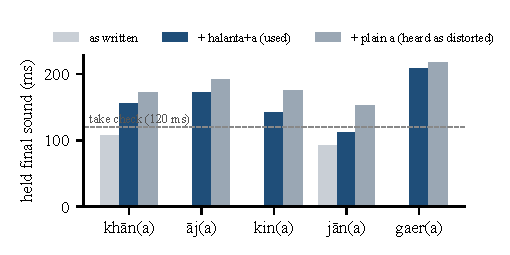
\includegraphics[width=\columnwidth]{fig_vowel.pdf}
\caption{Duration of the held word-final sound, forced alignment, 8 takes per spelling. Missing bars: not measured as written. The plain form was heard as distorted.}\label{fig:vowel}
\end{figure}

\paragraph{English.} Fig.~\ref{fig:english} compares four ways of producing full English sentences. English text with a Nepali prompt is unusable (best-take WER 59.5\%). English text with a prompt of the same speaker speaking English, found in the podcasts, is intelligible (5.8\%) and scores the highest UTMOS, but the native listener found it hard to understand. Nepali-letter English with the original spellings is intelligible to Whisper (0.3\%) yet was heard as broken, for example \emph{everyone} as ``eveeonee''. With the reviewed spellings every voice reaches 0.0\% on the best take, the line that failed for every voice before (\emph{bought a beautiful new jacket}) included, and the listener accepted it. Two English fine-tunes, LibriTTS-R speech paired with Nepali-letter text and the speakers' own 344 English clips, changed nothing measurable.

\begin{figure}[t]\centering
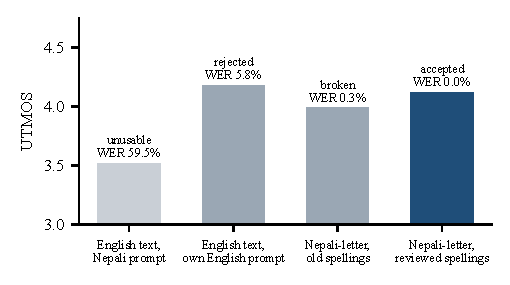
\includegraphics[width=\columnwidth]{fig_english.pdf}
\caption{Full English sentences: UTMOS, best-take Whisper WER and the native listener's verdict for four routes. The routes used different voices and numbers of takes (see text), so the figure compares routes, not voices.}\label{fig:english}
\end{figure}

\subsection{RQ4: Training vs Prompting}
Eight preset voices, four female and four male, come from one studio speaker and the permitted podcasts. Table~\ref{tab:pod} compares the base model with the model fine-tuned on the speakers' own podcast speech, on pieces held out from training. Similarity rises by 0.005 on average, pronunciation CER moves in both directions, and UTMOS is level; cloning of unseen speakers is unchanged (similarity 0.650 to 0.652, CER 6.4 to 6.3). Full fine-tunes on the two studio speakers gave the same picture (F0 correlation 0.42--0.47 against 0.49 for the base). The base model already clones these voices from a prompt; we keep the fine-tuned model because it is never worse.

\begin{table}[t]\centering\small
\caption{Clone against the speaker's real held-out piece, base / fine-tuned, 8 pieces per voice, one take (5 of 10 voices).}\label{tab:pod}
\begin{tabular}{lccc}\toprule
Voice & Similarity & Pron.\ CER & UTMOS\\\midrule
Podcast host (m) & .626 / .636 & 1.9 / 2.2 & 3.11 / 3.11\\
Guest 1 (m) & .753 / .760 & 3.6 / 2.1 & 3.54 / 3.52\\
Podcast host A (f) & .697 / .698 & 2.7 / 3.3 & 3.95 / 3.88\\
Interview A (f) & .725 / .729 & 3.3 / 3.2 & 3.76 / 3.89\\
Interview B (f) & .671 / .678 & 3.3 / 2.9 & 3.93 / 3.85\\\bottomrule
\end{tabular}
\end{table}

\subsection{Prompt Voice and Naturalness}\label{sec:voice}
Predicted naturalness depends mostly on the prompt. On 60 held-out Rasa sentences, the studio prompt gives UTMOS 3.55 and the podcast voices 3.89--3.95, at higher CER (6.9--7.2 against 4.6) because the podcast prompts are fast casual talk. A read-style prompt, made by letting the model read training-split sentences in the podcast voice and keeping the take that clones best on other training sentences, keeps the voice and lowers CER to 5.4--5.9 at UTMOS 4.07--4.16. Short phrases are the exception: F5 copies the prompt's pace, and on 40 short phrases (four seeds each) every podcast voice makes 40--80\% more errors than the studio voice (14.3--18.5 against 10.3) for $+0.2$ UTMOS; slowing the voice does not remove the gap. NepTTS-Bench is 94\% phrases under 30 letters, which is why the Maya and Sabina rows in Table~\ref{tab:bench} trade pronunciation for naturalness. Our own recogniser, Kriti, does not see this gap on the same audio (pronunciation CER 4.6 for the studio voice, 4.1--4.4 for the podcast voices), and neither did the native listener: in a blind choice over 12 short phrases, the studio voice was never preferred, Maya won 8 and Nisha 4; among male voices Aarav and Sujan won 5 each and the studio voice none. The short-phrase penalty is therefore at least partly MMS's, though the benchmark is scored with it. Maya and Aarav are the demo voices. Best-of-4 takes by our own recogniser, more flow steps, output enhancement (resemble-enhance~\citep{resembleenhance} raises UTMOS on long sentences by 0.24 but not on short phrases), loudness normalisation and silence padding did not change this.

\subsection{Human Evaluation}
A pilot with one native rater (17 sentences per system, 1--5 scale, loudness-matched) gave the human recordings 3.75, Swar 3.12, OmniVoice 3.06, Piper 3.06, TingTing 2.82 and ElevenLabs 2.76. A blind public listening test with naturalness and pronunciation ratings, A/B comparisons and a vote over the eight preset voices is built; its results will be added in a revision.

\section{Discussion}

\paragraph{Where the gains came from.} Every large improvement in this work came from the prompt, the text the model reads, or the choice among takes; none came from more training. Calm read prompts lowered benchmark CER from 35.2 to 11.8 early on, sentence chunking lowered paragraph CER from 15.7 to 5.4, and the frontend and take selection account for the rest of the pronunciation lead. Speaker fine-tunes, English fine-tunes, more data (338 h against 130 h), a higher learning rate, 64 flow steps, other guidance strengths, best-of-$N$ by another ASR or by NepaliMOS, punctuation restored from pauses (questions became flatter), training on BigVGAN mels, and DeepFilterNet on podcast audio (UTMOS $+0.0$ to $+0.2$: casual talk scores low, it is not noisy) did not help.

\paragraph{Objective scores and the listener.} Twice a native listener heard a problem the metrics could not see. The ASR read-back reported \np{खान} as correct while the vowel was missing, because its language model wrote the word it expected; only duration measurement showed it. For full English, the route with the best UTMOS and a low WER was the one the listener rejected, while the route the listener accepted differed from a rejected one only in spelling. Automatic scores were useful for ranking takes, but not for choosing between methods.

\paragraph{Limitations.} The held-vowel rule is a word list and will miss cases. The English review covers 2000 words; rules handle the rest and will be wrong for some. English from an upload that contains no English is weaker. The human evaluation so far is one rater. The UTMOS and NepaliMOS predictors were not trained on Nepali conversational speech.

\paragraph{Ethics.} Voice cloning can be misused. The demo asks the uploader to confirm that the speaker agreed. The podcast voices were used with permission, their audio is not released, and the preset names are ours, not the speakers'. Watermarking generated audio is future work.

\section{Conclusion}
Swar shows that an open model can speak Nepali the way it is spoken in Nepal and clone a voice from a short voice note. On NepTTS-Bench it makes the fewest pronunciation errors of any system, about two thirds of the next one's, and its demo voice scores the highest predicted naturalness. The largest gains came from writing the input the way it should sound, and from listening: the two most effective fixes started as a listener's report and were confirmed by measurement. We release the model, the frontend, the enrolment pipeline and the evaluation scripts.


\bibliographystyle{IEEEtranN}
\bibliography{refs}

\end{document}
